\section{Introduction}

Recently the Telecoms Regulator mandated a change to the way call costs are calculated for calls that cross peak/off-peak boundary's. Unfortunately the software system used by AcmeTelecom to calculate these changes has not been under active development. As a result of this, no current employees have experience or knowledge involving the current structure of the system. 

\subsection{Description of Change}
Currently, if a call is initiated during off-peak hours and continues into peak time, the whole call is charged at the off-peak rate. Conversely, if a call is initiated at peak time and continues to off-peak time the customer is charged at the peak rate for the whole call.

The Telecom Regulator has recently published a directive relating to the billing of calls that occur across peak/off-peak and off-peak/peak boundaries. This directive states that any customer who initiates a call during particular rate must only be charged at that rate until the time boundary for that rate is crossed.

We will assume Rate 1 is 12p per minute and Rate 2 is 8p per minute.

\begin{center}

  \begin{tabular}{ l | l  }
    Call A: 18:55 - 19:32 & Call B: 06:40 - 07:38 \\ \hline 
    Rate 1 - 6min = 12p * 6min = 72p & Rate 1 - 37min = 12p * 37min = 444p \\
    Rate 2 - 31min = 8p * 31min = 248p & Rate 2 - 21min = 8p * 21min = 168p \\
\hline
    Total = 72 + 248 = \textsterling 3.20 & Total = 444p + 168p = \textsterling 6.12 \\
  \end{tabular}
\end{center}


\subsection{Project Scope}

The new functionality will be incorporated in the Billing System which is contained in the com.acmetelecom package. Code from all other packages e.g. com.acmetelecom.customer will be considered out of scope. The diagram below illustrates the scope of the com.acmetelecom package. 

\begin{center}
	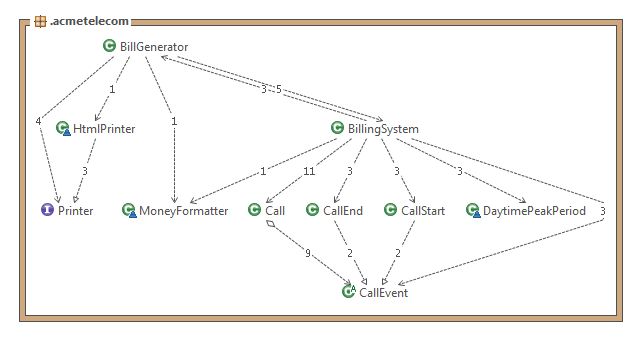
\includegraphics[scale=0.55]{images/Acme_Telecom_Structure.png}
\end{center}

